\section{Logistical Regression}
\subsection{Sigmoid}
Function which returns numbers between 0 and 1.
\[
\sigma(x) = \frac{1}{1 + e^{-x}} = \frac{e^x}{1 + e^x}
\]
\begin{center}
	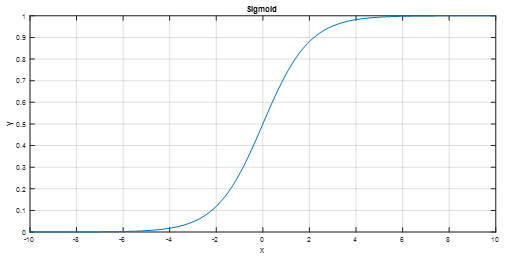
\includegraphics[width=0.6\columnwidth]{Images/sigmoid}
\end{center}
\textbf{Properties}:
\begin{align*}
	\sigma(0) &= 0.5 \\
	\sigma(-x) &=  1 - \sigma(x)\\
	\sigma'(x) &= \sigma(x)(1 - \sigma(x)) \\
	\int\sigma(x) dx &= \ln(1 + e^x) + const
\end{align*}